\chapter{Results}
In the following, we present the results we obtained by answering the Key Analytical Questions defined in Chapter \ref{ch:2} using the data warehouse designed and implemented in the previous chapters. For that, we executed the queries defined for each question against the data warehouse and visualized the results using appropriate charts.

\paragraph{How does user engagement evolve over multiple subscription tiers over time?}

For our first question, we wanted to know how the user engagement evolves over multiple subscription tiers. But it is also helpful to see how engagement evolves over time in general, so we can spot trends and seasonality. Therefore, we created a query that aggregates the number of active users per month and subscription tier. Furthermore, we also wanted to see how many active users are in each tier in total over the time span, so we can see, which tier has the most engagement. Finally, we wanted to know what the total engagement was over the total time span to see how many users were active in total. To extract those information, we used the query described in Listing \ref{lst:kaq1}.
\begin{lstlisting}[language=SQL,caption={Query for answering: How does user engagement evolve over time across subsciption tiers?},label={lst:kaq1},captionpos=b]
SELECT t.year, t.month, u.subscription_tier,
  SUM(f.active_user_flag) AS dau,
FROM fact_product_usage_engagement f
JOIN dim_time t ON t.time_key = f.time_key
JOIN dim_user u ON u.user_key = f.user_key
GROUP BY GROUPING SETS (
  (t.year, t.month, u.subscription_tier),
  (t.year, t.month),
  (u.subscription_tier),
  ()
)
ORDER BY t.year NULLS LAST, t.month NULLS LAST,
                u.subscription_tier NULLS LAST;
\end{lstlisting}

To retrieve the data we wanted to know, it was benefitial to use the \texttt{GROUPING SETS} feature of SQL, which allows us to group by multiple dimensions in a single query. This way, we could get the monthly active users per subscription tier, the total active users per subscription tier, and the total active users overall in a single query. After executing the query against our data warehouse, we visualized the results of the evolution of user engagement over time in Figure \ref{fig:kaq1}.
\begin{figure}[H]
    \centering
    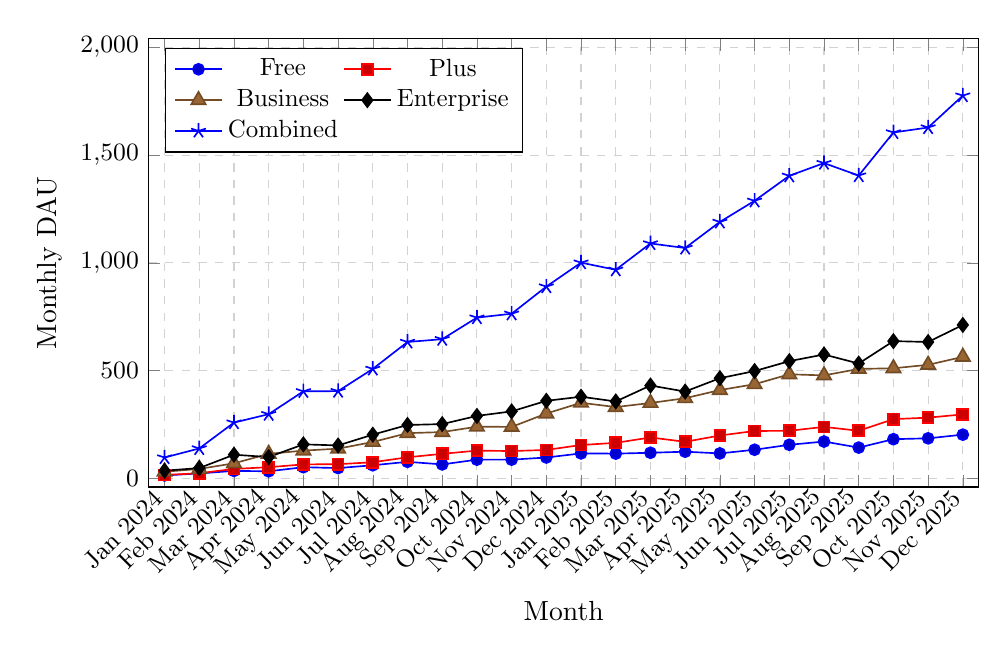
\begin{tikzpicture}
        \begin{axis}[
            width=\textwidth,
            height=0.6\textwidth,
            xlabel={Month},
            ylabel={Monthly DAU},
            xmin=1,
            xmax=24,
            ymin=0,
            ymax=2000,
            xtick={1,...,24},
            xticklabels={
                Jan 2024,Feb 2024,Mar 2024,Apr 2024,May 2024,Jun 2024,
                Jul 2024,Aug 2024,Sep 2024,Oct 2024,Nov 2024,Dec 2024,
                Jan 2025,Feb 2025,Mar 2025,Apr 2025,May 2025,Jun 2025,
                Jul 2025,Aug 2025,Sep 2025,Oct 2025,Nov 2025,Dec 2025
            },
            xticklabel style={rotate=45, anchor=east},
            tick label style={font=\small},
            legend style={at={(0.02,0.98)}, anchor=north west, nodes={scale=0.9, transform shape}},
            legend columns=2,
            grid=both,
            major grid style={dashed, gray!35},
            minor grid style={dotted, gray!20},
            enlargelimits=0.02,
            unbounded coords=discard
        ]
            \addplot+[semithick, mark=*, mark size=2pt] coordinates {
                (1, 14) (2, 23) (3, 35) (4, 33) (5, 52) (6, 48)
                (7, 61) (8, 77) (9, 65) (10, 87) (11, 87) (12, 97)
                (13, 116) (14, 115) (15, 119) (16, 124) (17, 116) (18, 133)
                (19, 156) (20, 171) (21, 143) (22, 182) (23, 186) (24, 203)
            };
            \addplot+[semithick, mark=square*, mark size=2pt] coordinates {
                (1, 16) (2, 24) (3, 44) (4, 52) (5, 65) (6, 66)
                (7, 75) (8, 98) (9, 114) (10, 129) (11, 127) (12, 132)
                (13, 155) (14, 165) (15, 190) (16, 170) (17, 199) (18, 220)
                (19, 221) (20, 239) (21, 221) (22, 275) (23, 282) (24, 297)
            };
            \addplot+[semithick, mark=triangle*, mark size=3pt] coordinates {
                (1, 31) (2, 44) (3, 70) (4, 114) (5, 129) (6, 138)
                (7, 169) (8, 210) (9, 215) (10, 240) (11, 239) (12, 301)
                (13, 351) (14, 331) (15, 350) (16, 372) (17, 410) (18, 437)
                (19, 483) (20, 478) (21, 508) (22, 511) (23, 527) (24, 564)
            };
            \addplot+[semithick, mark=diamond*, mark size=2.5pt] coordinates {
                (1, 36) (2, 48) (3, 110) (4, 99) (5, 158) (6, 153)
                (7, 203) (8, 248) (9, 252) (10, 290) (11, 311) (12, 360)
                (13, 379) (14, 357) (15, 431) (16, 403) (17, 465) (18, 498)
                (19, 544) (20, 575) (21, 533) (22, 637) (23, 633) (24, 712)
            };
            \addplot+[semithick, mark=star, mark size=2.8pt] coordinates {
                (1, 97) (2, 139) (3, 259) (4, 298) (5, 404) (6, 405)
                (7, 508) (8, 633) (9, 646) (10, 746) (11, 764) (12, 890)
                (13, 1001) (14, 968) (15, 1090) (16, 1069) (17, 1190) (18, 1288)
                (19, 1404) (20, 1463) (21, 1405) (22, 1605) (23, 1628) (24, 1776)
            };
            \legend{Free, Plus, Business, Enterprise, Combined}
        \end{axis}
    \end{tikzpicture}
    \caption{Monthly DAU by subscription tier for Jan 2024--Dec 2025.}
    \label{fig:kaq1-dau}
\end{figure}
